\documentclass[tikz,border=8pt]{standalone}
% Shared look for every TikZ diagram. Load with \input{../../tools/tikz-style.tex}
\usepackage[T1]{fontenc}
\usepackage{lmodern}
\renewcommand{\sfdefault}{lmr}  % diagrams use the same serif as the text
\usetikzlibrary{arrows.meta, positioning, shapes.geometric, calc, fit, backgrounds}
\definecolor{cblue}{HTML}{4C78A8}
\definecolor{corange}{HTML}{F58518}
\definecolor{cgreen}{HTML}{54A24B}
\definecolor{cred}{HTML}{E45756}
\definecolor{cpurple}{HTML}{B279A2}
\definecolor{cgrey}{HTML}{6B6B6B}
\tikzset{
  every picture/.style={font=\sffamily, line width=1.2pt},
  box/.style={draw=#1, fill=#1!12, rounded corners=4pt, align=center, inner sep=7pt, minimum height=1.1cm},
  box/.default=cgrey,
  arrow/.style={-{Stealth[length=3mm]}, draw=cgrey, line width=1.4pt},
  title/.style={font=\sffamily\bfseries\Large},
  note/.style={font=\sffamily\small, text=cgrey, align=center},
}
\AtBeginDocument{\hyphenpenalty=10000 \exhyphenpenalty=10000}

\begin{document}
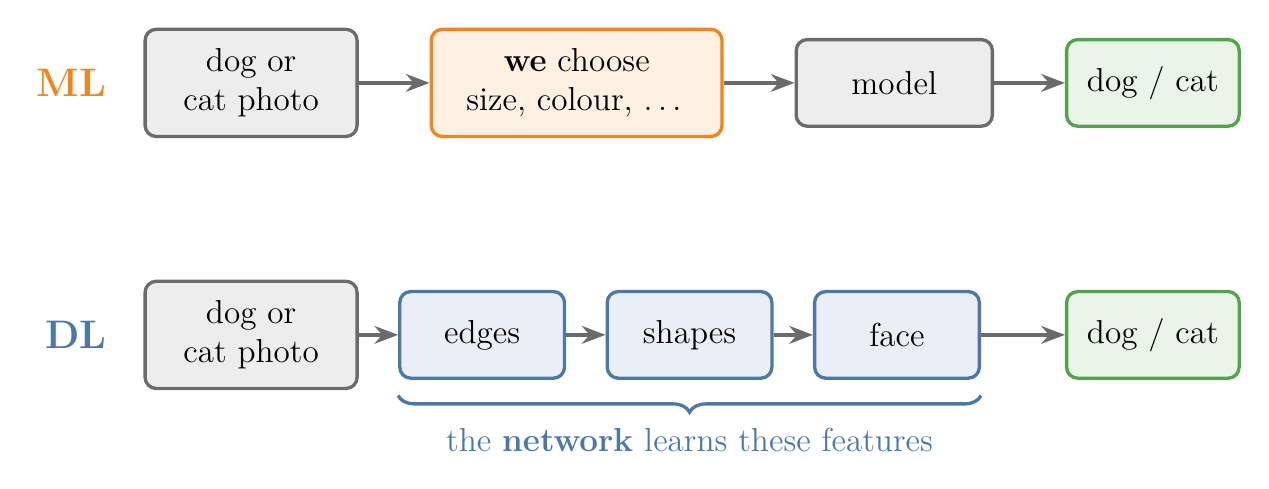
\begin{tikzpicture}[every node/.append style={font=\sffamily\large}, node distance=0.9cm]
  % ML row
  \node[font=\sffamily\bfseries\Large, text=corange, anchor=east] at (-0.4,0) {ML};
  \node[box=cgrey, text width=2.2cm] (r1) at (1.3,0) {dog or\\cat photo};
  \node[box=corange, text width=3.2cm, right=of r1] (f1) {\textbf{we} choose\\size, colour, \dots};
  \node[box=cgrey, text width=2.0cm, right=of f1] (m1) {model};
  \node[box=cgreen, text width=1.7cm, right=of m1] (o1) {dog / cat};
  \draw[arrow] (r1) -- (f1); \draw[arrow] (f1) -- (m1); \draw[arrow] (m1) -- (o1);
  % DL row
  \node[font=\sffamily\bfseries\Large, text=cblue, anchor=east] at (-0.4,-3.2) {DL};
  \node[box=cgrey, text width=2.2cm] (r2) at (1.3,-3.2) {dog or\\cat photo};
  \node[box=cblue, text width=1.6cm, right=0.5cm of r2] (l1) {edges};
  \node[box=cblue, text width=1.6cm, right=0.5cm of l1] (l2) {shapes};
  \node[box=cblue, text width=1.6cm, right=0.5cm of l2] (l3) {face};
  \node[box=cgreen, text width=1.7cm] (o2) at (o1 |- l3) {dog / cat};
  \draw[arrow] (r2) -- (l1); \draw[arrow] (l1) -- (l2); \draw[arrow] (l2) -- (l3); \draw[arrow] (l3) -- (o2);
  \draw[decorate, decoration={brace, amplitude=6pt, mirror}, draw=cblue] (l1.south west) ++(0,-0.2) -- ($(l3.south east)+(0,-0.2)$)
    node[midway, below=8pt, text=cblue] {the \textbf{network} learns these features};
\end{tikzpicture}
\end{document}
